% !TEX root = ../main.tex
\section{Method}
\label{sec:method}

We model the interaction as nested Markov chains (Figure~\ref{fig:nested-markov}) and generate synthetic dialogues by sampling a per-trajectory user profile, state transitions, and a quality signal, then conditioning an LLM on the resulting latent state to produce user and assistant messages. The user and quality model is in \S\ref{sec:method:user}, the chain structure in \S\ref{sec:method:model}, state sampling in \S\ref{sec:method:transitions}, the generation loop in \S\ref{sec:method:generation}, and theoretical outcome and length distributions in \S\ref{sec:method:theory}.

\begin{figure}[t]
  \centering
  \adjustbox{width=\linewidth}{\adjustbox{trim={.05\width} 0 {.05\width} 0, clip}{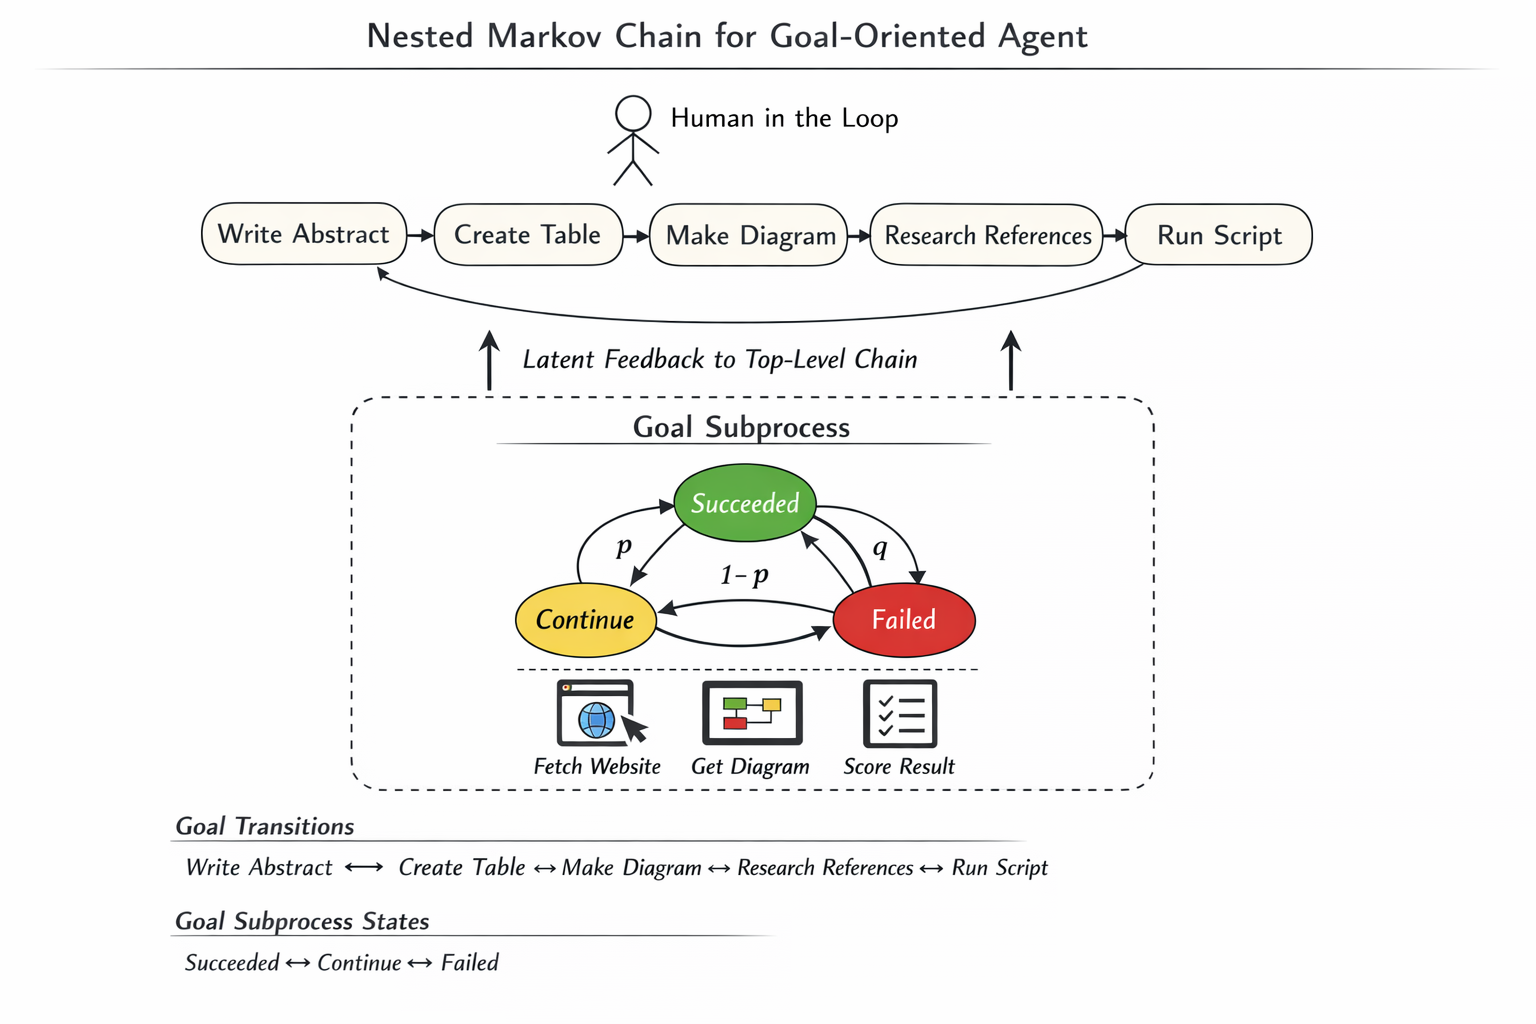
\includegraphics{figures/nested_markov_chain.png}}}
  \caption{Nested Markov chain: top layer includes start, goals (e.g.\ writing-assistant tasks), outcome states (publish, subscribe), and terminals (finished, abandoned); one goal is expanded to show the per-goal sub-chain (continue, succeeded, failed). Goal-specific tools influence nested transitions; latent feedback influences the top-level chain.}
  \label{fig:nested-markov}
\end{figure}

% -----------------------------------------------------------------------------
\subsection{User profile and quality distribution}
\label{sec:method:user}
% -----------------------------------------------------------------------------

At the beginning of each trajectory we draw a single multivariate \emph{user profile} $\mathbf{u}$ that stays fixed for that user and determines dialogue style and how they respond to success or failure. We use a four-dimensional vector:
\begin{equation}
  \mathbf{u} = (u_{\mathrm{tech}}, u_{\mathrm{det}}, u_{\mathrm{swear}}, u_{\mathrm{sent}}) \sim p(\mathbf{u}), \label{eq:user-draw}
\end{equation}
where $u_{\mathrm{tech}}$ encodes how technical the user is, $u_{\mathrm{det}}$ how determined (persistent), $u_{\mathrm{swear}}$ how easily they swear when frustrated, and $u_{\mathrm{sent}}$ their baseline sentiment (high = more positive). For example, $\mathbf{u} \sim \mathcal{N}(\boldsymbol{\mu}_u, \boldsymbol{\Sigma}_u)$ with bounds or truncation so components lie in $[0,1]$ or a finite range. This profile is passed into the LLM prompt so that generated messages match the user type.

\paragraph{Quality signal.}
At each step $t$ we draw a scalar quality $z_t$ that drives the tone of the turn (satisfaction or frustration). When in a goal with nested state $x_t$, the quality depends on $x_t$ and the user's baseline sentiment:
\begin{equation}
  z_t \sim \mathcal{N}\bigl(\mu(x_t) + \lambda_{\mathrm{sent}} u_{\mathrm{sent}},\; \sigma^2\bigr), \qquad \mu \colon \mathcal{X} \to \mathbb{R}, \quad \sigma^2 > 0. \label{eq:quality}
\end{equation}
E.g., $\mu(\mathsf{succeeded}) > \mu(\mathsf{continue}) > \mu(\mathsf{failed})$. When $s_t \notin \mathcal{G}$, we take $z_t \sim \mathcal{N}(\mu_0 + \lambda_{\mathrm{sent}} u_{\mathrm{sent}}, \sigma^2)$. The value $z_t$ is injected into the LLM prompt so that user and assistant messages match the intended quality level.

\paragraph{Dependence of nested chain on user and tool quality.}
The nested transition kernel for goal $g$ depends on the user profile $\mathbf{u}$ and on a \emph{tool quality} parameter $q_g \in \mathbb{R}$ (e.g., higher $q_g$ = better tool for that goal). We write
\begin{equation}
  x_{t+1} \sim \pi_g(\cdot \mid x_t; \mathbf{u}, q_g). \label{eq:nested-user-tool}
\end{equation}
A simple and interpretable assumption is to make the probability of favourable transitions increase with determination and tool quality. For example, from $\mathsf{continue}$, the probability of moving to $\mathsf{succeeded}$ rather than $\mathsf{failed}$ can be modelled with a logit-linear form:
\begin{equation}
  \mathbb{P}(x_{t+1} = \mathsf{succeeded} \mid x_t = \mathsf{continue}; \mathbf{u}, q_g) = \sigma\bigl(\alpha_g + \beta_{\mathrm{det}} u_{\mathrm{det}} + \gamma_g q_g\bigr), \label{eq:nested-logit}
\end{equation}
where $\sigma$ is the logistic function, $\alpha_g$ is a goal-specific intercept, and $\beta_{\mathrm{det}}, \gamma_g$ are coefficients. So more determined users and better tools increase the chance of success from the continue state; the converse can be assumed for $\mathsf{failed}$. Other transitions (e.g., from $\mathsf{succeeded}$ or $\mathsf{failed}$ back to $\mathsf{continue}$) can be parametrised similarly as functions of $\mathbf{u}$ and $q_g$, with constraints so that each row of the transition matrix sums to one. This yields a nested chain that is user- and tool-dependent while remaining tractable.

% -----------------------------------------------------------------------------
\subsection{Nested Markov model}
\label{sec:method:model}
% -----------------------------------------------------------------------------

\paragraph{Top-level chain.}
The top-level state space is
\begin{equation}
  \mathcal{S} = \{\mathsf{start}\} \cup \mathcal{G} \cup \{\mathsf{publish},\mathsf{subscribe}\} \cup \{\mathsf{finished},\mathsf{abandoned}\},
\end{equation}
where $\mathcal{G}$ is a finite set of goal states. The top-level dynamics are given by a transition kernel $\pi_{\mathrm{top}}$ that may depend on the nested outcome when in a goal:
\begin{equation}
  s_{t+1} \sim \pi_{\mathrm{top}}(\cdot \mid s_t, x_{t+1}), \qquad s_t, s_{t+1} \in \mathcal{S}
\end{equation}
(with $x_{t+1}$ irrelevant when $s_t \notin \mathcal{G}$). The states $\mathsf{finished}$ and $\mathsf{abandoned}$ are absorbing: once $s_t \in \{\mathsf{finished},\mathsf{abandoned}\}$, the trajectory stops.

\paragraph{Nested chain (per goal).}
For each goal $g \in \mathcal{G}$, the nested state space is $\mathcal{X} = \{\mathsf{succeeded},\mathsf{continue},\mathsf{failed}\}$. When $s_t = g$, we maintain $x_t \in \mathcal{X}$. The nested kernel $\pi_g(\cdot \mid x_t; \mathbf{u}, q_g)$ is as in \eqref{eq:nested-user-tool}--\eqref{eq:nested-logit}, depending on the user profile $\mathbf{u}$ and tool quality $q_g$. The outcome $x_{t+1}$ influences the next top-level state (e.g., succeeded $\to$ higher mass on publish/finished; failed $\to$ higher mass on abandoned).

% -----------------------------------------------------------------------------
\subsection{State transition sampling}
\label{sec:method:transitions}
% -----------------------------------------------------------------------------

At each step $t$, the next state is drawn as follows.

\begin{itemize}
  \item \textbf{If $s_t \in \mathcal{G}$:} First sample the nested transition (using the current user $\mathbf{u}$ and tool quality $q_{s_t}$), then the top-level transition:
  \begin{align}
    x_{t+1} &\sim \pi_{s_t}(\cdot \mid x_t; \mathbf{u}, q_{s_t}), \label{eq:nested-draw} \\
    s_{t+1} &\sim \pi_{\mathrm{top}}(\cdot \mid s_t, x_{t+1}). \label{eq:top-draw}
  \end{align}

  \item \textbf{If $s_t \in \mathcal{S} \setminus \mathcal{G}$:} There is no nested state; draw only the top-level transition:
  \begin{equation}
    s_{t+1} \sim \pi_{\mathrm{top}}(\cdot \mid s_t). \label{eq:top-only}
  \end{equation}
\end{itemize}

% -----------------------------------------------------------------------------
\subsection{Trajectory generation}
\label{sec:method:generation}
% -----------------------------------------------------------------------------

We draw $\mathbf{u} \sim p(\mathbf{u})$ once per trajectory. We maintain latent state $(s_t, x_t, z_t)$ (with $x_t$ defined only when $s_t \in \mathcal{G}$).

At each step $t$:
\begin{enumerate}
  \item Sample $(s_{t+1}, x_{t+1})$ from the Markov chains as in \S\ref{sec:method:transitions} (\ref{eq:nested-draw})--(\ref{eq:top-only}).
  \item Sample quality $z_{t+1}$ from \eqref{eq:quality} (or the default Gaussian when not in a goal).
  \item Build a prompt encoding the new latent state, user profile $\mathbf{u}$, and $z_{t+1}$. Call the LLM twice to generate the user message and the assistant response.
  \item Set $t \leftarrow t+1$ and repeat until $s_t \in \{\mathsf{finished},\mathsf{abandoned}\}$.
\end{enumerate}

Generation stops as soon as the top-level state is $\mathsf{finished}$ or $\mathsf{abandoned}$.

% -----------------------------------------------------------------------------
\subsection{Theoretical outcome and trajectory-length distributions}
\label{sec:method:theory}
% -----------------------------------------------------------------------------

Under a fixed user $\mathbf{u}$ and fixed tool qualities $\{q_g\}$, the joint process over $(s_t, x_t)$ is a discrete-time Markov chain on the product space of top-level and (when applicable) nested states. The top-level chain alone, when marginalised over the nested outcomes, is generally not Markov; however, if we condition on $\mathbf{u}$ and $\{q_g\}$, we can still analyse absorption and hitting probabilities by viewing the effective top-level dynamics as a (larger) Markov chain whose states encode the current goal and nested state, or by Monte Carlo. Below we give the form of the theoretical quantities when the effective dynamics are Markov (e.g., if we fix a single goal or collapse the nested chain to a summary state).

\paragraph{Absorption and hitting probabilities.}
Let the transient states be $\mathcal{T} = \mathcal{S} \setminus \{\mathsf{finished},\mathsf{abandoned}\}$. Order states so that transient states come first, then $\mathsf{finished}$, then $\mathsf{abandoned}$. The one-step transition matrix on $\mathcal{S}$ can be written in block form:
\begin{equation}
  \mathbf{P} = \begin{bmatrix} \mathbf{Q} & \mathbf{R} \\ \mathbf{0} & \mathbf{I} \end{bmatrix},
\end{equation}
where $\mathbf{Q}$ is the restriction to $\mathcal{T} \times \mathcal{T}$, $\mathbf{R}$ is $\mathcal{T} \times \{\mathsf{finished},\mathsf{abandoned}\}$, and $\mathbf{I}$ is the $2\times 2$ identity. The \emph{fundamental matrix} is $\mathbf{N} = (\mathbf{I} - \mathbf{Q})^{-1}$ (well-defined if absorption is almost sure from every transient state) \citep{kemeny1976finite, norris1997markov}. Let $\boldsymbol{\alpha}$ be the initial distribution over $\mathcal{T}$ (e.g., point mass on $\mathsf{start}$). The probability of eventually being absorbed in $\mathsf{finished}$ vs $\mathsf{abandoned}$ is
\begin{equation}
  \mathbb{P}(\mathsf{finished}) = \boldsymbol{\alpha}' \mathbf{N} \mathbf{R}_{\mathsf{finished}}, \qquad \mathbb{P}(\mathsf{abandoned}) = \boldsymbol{\alpha}' \mathbf{N} \mathbf{R}_{\mathsf{abandoned}}, \label{eq:absorb-prob}
\end{equation}
where $\mathbf{R}_{\mathsf{finished}}$ and $\mathbf{R}_{\mathsf{abandoned}}$ are the columns of $\mathbf{R}$ corresponding to each absorbing state. The probability of \emph{ever visiting} a given outcome state (e.g., $\mathsf{publish}$ or $\mathsf{subscribe}$) before absorption can be obtained similarly by treating that state as a (virtual) absorbing target and solving the hitting-probability linear system: if $\mathcal{H}$ is the set of states that count as ``hit'' (e.g., $\mathsf{publish}$), then the vector $\mathbf{h}$ of hitting probabilities from each transient state satisfies $\mathbf{h} = \mathbf{r} + \mathbf{Q}\mathbf{h}$ on transient states (with boundary conditions $h_i = 1$ for $i \in \mathcal{H}$, $h_i = 0$ for other absorbing states), yielding a closed-form linear system $\mathbf{h} = (\mathbf{I}-\mathbf{Q})^{-1}\mathbf{r}$ when the target set is appropriately encoded in $\mathbf{r}$.

\paragraph{Trajectory length.}
Let $T$ be the first time $t$ such that $s_t \in \{\mathsf{finished},\mathsf{abandoned}\}$. The distribution of $T$ is a discrete phase-type distribution \citep{neuts1981matrix}. The probability that absorption has not occurred by step $t$ is
\begin{equation}
  \mathbb{P}(T > t) = \boldsymbol{\alpha}' \mathbf{Q}^t \mathbf{1}, \label{eq:survival}
\end{equation}
so $\mathbb{P}(T = t) = \boldsymbol{\alpha}' \mathbf{Q}^{t-1}(\mathbf{I}-\mathbf{Q})\mathbf{1}$ for $t \geq 1$ (with the convention that $\mathbf{Q}^0 = \mathbf{I}$). The expected trajectory length is
\begin{equation}
  \mathbb{E}[T] = \boldsymbol{\alpha}' \mathbf{N} \mathbf{1}. \label{eq:expected-length}
\end{equation}
Higher moments (e.g., $\mathbb{E}[T^2]$) can be obtained from the moment-generating function or from $\mathbf{N}^2$ and higher powers. Thus the full distribution and moments are available in closed form in terms of $\mathbf{Q}$, $\mathbf{N}$, and $\boldsymbol{\alpha}$. When the effective top-level process is not exactly Markov (because of the nested chain), the same formulas apply to the \emph{augmented} chain whose states are $(s_t, x_t)$ (or a finite aggregation thereof), with $\mathbf{Q}$ and $\mathbf{R}$ defined on that augmented space; alternatively, one can approximate by averaging over the stationary distribution of the nested chain per goal to get an effective $\mathbf{Q}$ and then use \eqref{eq:absorb-prob}--\eqref{eq:expected-length} as an approximation.

\paragraph{Integrating over the user distribution.}
All of the above quantities depend on $\mathbf{u}$ (and on $\{q_g\}$) through $\mathbf{Q}$ and $\mathbf{R}$. Denote by $\mathbb{P}(\cdot \mid \mathbf{u}, \mathbf{q})$, $\mathbb{E}[T \mid \mathbf{u}, \mathbf{q}]$, etc., the absorption probabilities, hitting probabilities, and expected length for a fixed user $\mathbf{u}$ and tool-quality vector $\mathbf{q}$. The \emph{population-level} quantities under the user distribution $p(\mathbf{u})$ are
\begin{align}
  \mathbb{P}(\mathsf{finished}) &= \int \mathbb{P}(\mathsf{finished} \mid \mathbf{u}, \mathbf{q})\, p(\mathbf{u})\, \mathrm{d}\mathbf{u}, \quad \text{and similarly for }\mathsf{abandoned},\ \mathsf{publish},\ \mathsf{subscribe}; \label{eq:pop-absorb} \\
  \mathbb{E}[T] &= \int \mathbb{E}[T \mid \mathbf{u}, \mathbf{q}]\, p(\mathbf{u})\, \mathrm{d}\mathbf{u}. \label{eq:pop-length}
\end{align}
Closed-form integration is possible only in special cases (e.g., conjugate $p(\mathbf{u})$ and a parametrisation that keeps the integrand in a simple form). In general, one approximates by Monte Carlo: draw $\mathbf{u}^{(1)}, \ldots, \mathbf{u}^{(M)} \sim p(\mathbf{u})$, compute $\mathbb{P}(\mathsf{finished} \mid \mathbf{u}^{(m)}, \mathbf{q})$ and the other quantities for each $m$ (via the fundamental matrix for the augmented chain under $\mathbf{u}^{(m)}$), and average. The same applies to $\mathbb{P}(\mathsf{publish})$, $\mathbb{P}(\mathsf{subscribe})$, and $\mathbb{E}[T]$.

\paragraph{Conditional probabilities and correlation.}
Let $Y_{\mathsf{pub}} = \mathbf{1}[\text{trajectory ever hits }\mathsf{publish}]$ and $Y_{\mathsf{sub}} = \mathbf{1}[\text{trajectory ever hits }\mathsf{subscribe}]$. The probability of subscribing given the user published \emph{exactly once} is
\begin{equation}
  \mathbb{P}(Y_{\mathsf{sub}} = 1 \mid \text{hit }\mathsf{publish}\text{ exactly once}) = \frac{\mathbb{P}(Y_{\mathsf{sub}} = 1,\, \text{hit }\mathsf{publish}\text{ exactly once})}{\mathbb{P}(\text{hit }\mathsf{publish}\text{ exactly once})}. \label{eq:sub-given-pub-once}
\end{equation}
Both numerator and denominator can be computed on an \emph{augmented} state space that records how many times $\mathsf{publish}$ (and optionally $\mathsf{subscribe}$) has been visited so far; the transition structure remains Markov on this augmented space, so the probabilities are given by the same fundamental-matrix and hitting-probability formalism. More generally, $\mathbb{P}(Y_{\mathsf{sub}} = 1 \mid \text{hit }\mathsf{publish}\text{ exactly }N\text{ times})$ is obtained by conditioning on the event that the count of visits to $\mathsf{publish}$ equals $N$ before absorption, which again reduces to linear algebra on the augmented chain. The \emph{correlation} between subscription and publish is
\begin{equation}
  \rho = \frac{\mathbb{P}(Y_{\mathsf{sub}} = 1,\, Y_{\mathsf{pub}} = 1) - \mathbb{P}(Y_{\mathsf{sub}} = 1)\mathbb{P}(Y_{\mathsf{pub}} = 1)}{\sqrt{\mathrm{Var}(Y_{\mathsf{sub}})\,\mathrm{Var}(Y_{\mathsf{pub}})}}, \label{eq:correlation}
\end{equation}
where $\mathrm{Var}(Y_{\mathsf{pub}}) = \mathbb{P}(Y_{\mathsf{pub}} = 1)(1 - \mathbb{P}(Y_{\mathsf{pub}} = 1))$ and similarly for $Y_{\mathsf{sub}}$; the joint probability $\mathbb{P}(Y_{\mathsf{sub}} = 1,\, Y_{\mathsf{pub}} = 1)$ is the probability of hitting both states before absorption, computable on the augmented chain that tracks whether each has been hit. All of these can be integrated over $p(\mathbf{u})$ as in \eqref{eq:pop-absorb} to obtain population-level conditional probabilities and correlation.

\paragraph{Comparing two systems (tool qualities $q_1 \neq q_2$).}
For a randomly drawn user $\mathbf{u} \sim p(\mathbf{u})$, the subscribe probability under tool quality $q$ is $p_{\mathsf{sub}}(\mathbf{u}; q) = \mathbb{P}(Y_{\mathsf{sub}} = 1 \mid \mathbf{u}, \mathbf{q}\big|_{q_g = q})$. This is a random variable when $\mathbf{u}$ is random. The probability that tool~2 leads to more subscriptions than tool~1 (for a random user) is
\begin{equation}
  \mathbb{P}\bigl(p_{\mathsf{sub}}(\mathbf{u}; q_2) > p_{\mathsf{sub}}(\mathbf{u}; q_1)\bigr) = \int \mathbf{1}\bigl[p_{\mathsf{sub}}(\mathbf{u}; q_2) > p_{\mathsf{sub}}(\mathbf{u}; q_1)\bigr]\, p(\mathbf{u})\, \mathrm{d}\mathbf{u}. \label{eq:prob-q2-beats-q1}
\end{equation}
Closed form is rarely available; the integral is approximated by Monte Carlo: draw $\mathbf{u}^{(m)} \sim p(\mathbf{u})$, compute $p_{\mathsf{sub}}(\mathbf{u}^{(m)}; q_1)$ and $p_{\mathsf{sub}}(\mathbf{u}^{(m)}; q_2)$ (e.g., from the fundamental matrix for each $\mathbf{q}$), and estimate the probability as the fraction of draws for which $p_{\mathsf{sub}}(\mathbf{u}^{(m)}; q_2) > p_{\mathsf{sub}}(\mathbf{u}^{(m)}; q_1)$.

\paragraph{Sample size to conclude that $q_2$ is better than $q_1$ at $X\%$ confidence.}
Suppose we run $N$ independent trajectories under system $q_1$ and $N$ under $q_2$, with users drawn i.i.d.\ from $p(\mathbf{u})$ for each trajectory. Let $\widehat{p}_1$ and $\widehat{p}_2$ be the empirical subscribe rates. We want the smallest $N$ such that a one-sided test of $H_0: \mu_1 \geq \mu_2$ vs $H_1: \mu_2 > \mu_1$ (where $\mu_q = \mathbb{E}_{\mathbf{u}}[p_{\mathsf{sub}}(\mathbf{u}; q)]$) has confidence (rejection of $H_0$ when true) at level $\alpha$ (e.g., $5\%$) and power $1 - \beta$ (e.g., $80\%$) when $\mu_2 - \mu_1 = \delta > 0$. Under a normal approximation for $\widehat{p}_1$ and $\widehat{p}_2$ (justified for large $N$ by the central limit theorem),
\begin{equation}
  N \geq \frac{(z_{\alpha} + z_{\beta})^2\, (\sigma_1^2 + \sigma_2^2)}{\delta^2}. \label{eq:sample-size}
\end{equation}
Here $z_{\alpha}$ and $z_{\beta}$ are the $\alpha$ and $\beta$ quantiles of the standard normal; $\sigma_q^2 = \mathrm{Var}_{\mathbf{u}}[p_{\mathsf{sub}}(\mathbf{u}; q)] + \mathbb{E}_{\mathbf{u}}[p_{\mathsf{sub}}(\mathbf{u}; q)(1 - p_{\mathsf{sub}}(\mathbf{u}; q))]/N \approx \mathrm{Var}_{\mathbf{u}}[p_{\mathsf{sub}}(\mathbf{u}; q)]$ for large $N$. The mean $\mu_q$ and variance $\mathrm{Var}_{\mathbf{u}}[p_{\mathsf{sub}}(\mathbf{u}; q)]$ are determined by the nested transition probabilities under $q$ and the user distribution $p(\mathbf{u})$; they can be computed in closed form only in special cases, and otherwise by Monte Carlo over $\mathbf{u}$. Given $\mu_1$, $\mu_2$, $\sigma_1^2$, $\sigma_2^2$ (from the model), \eqref{eq:sample-size} yields the required $N$ per system so that at $X\%$ confidence (e.g., $1-\alpha = 95\%$) we can detect that $q_2$ is better than $q_1$ with the desired power.

\paragraph{Using publish as a proxy for subscribe: smaller sample size.}
In practice, users often \emph{publish} multiple times per trajectory (or at least hit $\mathsf{publish}$ more often) while they \emph{subscribe} at most once; subscribe is the rarer, primary outcome. If publish and subscribe are positively correlated ($\rho > 0$), we can use the difference in \emph{publish} rates (or ``ever publish'') as a proxy for the difference in subscribe rates. Testing $H_0: \mu_{\mathsf{pub}}^{(q_1)} = \mu_{\mathsf{pub}}^{(q_2)}$ instead of $H_0: \mu_{\mathsf{sub}}^{(q_1)} = \mu_{\mathsf{sub}}^{(q_2)}$ can then yield significant results with a \emph{smaller} sample size when the standardized effect size on the proxy is larger than on the target. The sample size per system when using the proxy is
\begin{equation}
  N_{\mathsf{pub}} \geq \frac{(z_{\alpha} + z_{\beta})^2\, (\sigma_{\mathsf{pub},q_1}^2 + \sigma_{\mathsf{pub},q_2}^2)}{\delta_{\mathsf{pub}}^2}, \qquad \delta_{\mathsf{pub}} = \mu_{\mathsf{pub}}^{(q_2)} - \mu_{\mathsf{pub}}^{(q_1)},
\end{equation}
with $\mu_{\mathsf{pub}}^{(q)}$, $\sigma_{\mathsf{pub},q}^2$ the mean and variance of $Y_{\mathsf{pub}}$ under tool quality $q$ (computable from the chain as in \eqref{eq:fp-hit} and \eqref{eq:fp-moments} with publish in place of subscribe). The \emph{ratio} of the sample size needed for subscribe vs.\ for the proxy is
\begin{equation}
  \frac{N_{\mathsf{sub}}}{N_{\mathsf{pub}}} = \frac{(\sigma_{\mathsf{sub},q_1}^2 + \sigma_{\mathsf{sub},q_2}^2)/\delta_{\mathsf{sub}}^2}{(\sigma_{\mathsf{pub},q_1}^2 + \sigma_{\mathsf{pub},q_2}^2)/\delta_{\mathsf{pub}}^2}.
\end{equation}
If this ratio exceeds $1$, we need fewer trajectories to detect a significant effect when using publish as the outcome. That happens when the effect on publish is proportionally larger (e.g., $\delta_{\mathsf{pub}}/\mu_{\mathsf{pub}} > \delta_{\mathsf{sub}}/\mu_{\mathsf{sub}}$) or when the variance of the publish outcome is smaller relative to $\delta_{\mathsf{pub}}$. Under the finite-persona model (\S\ref{sec:method:finite-personas}), $\mu_{\mathsf{pub}}^{(q)}$, $\sigma_{\mathsf{pub},q}^2$, $\delta_{\mathsf{pub}}$, and the correlation $\rho$ between $Y_{\mathsf{pub}}$ and $Y_{\mathsf{sub}}$ are all closed form; we can therefore compute $N_{\mathsf{pub}}$ and $N_{\mathsf{sub}}$ and the ratio exactly. When $\rho$ is high, a significant increase in publish under $q_2$ vs $q_1$ is strong evidence that subscribe also increases; when $\rho$ is moderate, the proxy test is conservative (it may reject for publish while subscribe is not yet significant) or can be combined with a small subsample where subscribe is observed to calibrate the relationship.

\paragraph{Special cases: factorized transitions and simple user distributions.}
Two assumptions make closed-form or tractable computation possible across the quantities above.

\textbf{Factorized transition probabilities.} Assume that the nested (and, when applicable, top-level) transition probabilities factorize into user- and tool-dependent parts, so that tool quality impacts all users in the same way. For the nested chain, this means for each goal $g$ and transition $x \to x'$ we have
\begin{equation}
  \pi_g(x' \mid x; \mathbf{u}, q_g) = \frac{\phi_g(x', x; \mathbf{u})\, \psi_g(x', x; q_g)}{Z_g(x; \mathbf{u}, q_g)}, \label{eq:factorize}
\end{equation}
where $\phi_g \geq 0$ depends only on the user, $\psi_g \geq 0$ only on the tool quality, and $Z_g$ is the normalising constant. Equivalently, in logit space we may assume $\mathrm{logit}\,\pi_g(x' \mid x; \mathbf{u}, q_g) = A_g(x', x; \mathbf{u}) + B_g(x', x; q_g)$, so that the effect of $q_g$ is a fixed shift for every user. Then, for a fixed user $\mathbf{u}$, the chain under tool quality $q$ is Markov with transition matrix determined by $\mathbf{u}$ and $q$; and when we integrate over $\mathbf{u}$, the dependence on $q$ separates from the user average in a structured way (e.g., expected outcomes under $q$ can be written as a sum over user types of a product of a user-term and a tool-term when the state space is small).

\textbf{Simple user distribution.} Assume users are drawn from a \emph{finite set of personas} $\{\mathbf{u}_1, \ldots, \mathbf{u}_K\}$ with probabilities $p_1, \ldots, p_K$, or from a distribution that yields simple integrals (e.g., conjugate priors so that expectations over $\mathbf{u}$ remain in closed form). Under a finite number of personas, all population integrals reduce to finite sums: $\mathbb{P}(\mathsf{finished}) = \sum_{k=1}^K p_k\, \mathbb{P}(\mathsf{finished} \mid \mathbf{u}_k, \mathbf{q})$, and each term is closed form via the fundamental matrix for the chain under $(\mathbf{u}_k, \mathbf{q})$. The same holds for $\mathbb{P}(\mathsf{abandoned})$, $\mathbb{P}(\mathsf{publish})$, $\mathbb{P}(\mathsf{subscribe})$, $\mathbb{E}[T]$, the conditional probabilities \eqref{eq:sub-given-pub-once} and correlation \eqref{eq:correlation}, and for $\mu_q$, $\sigma_q^2$ in the sample-size formula \eqref{eq:sample-size}. The probability that tool~2 leads to more subscriptions than tool~1 becomes $\mathbb{P}(p_{\mathsf{sub}}(\mathbf{u}; q_2) > p_{\mathsf{sub}}(\mathbf{u}; q_1)) = \sum_{k:\, p_{\mathsf{sub}}(\mathbf{u}_k; q_2) > p_{\mathsf{sub}}(\mathbf{u}_k; q_1)} p_k$, which is a closed-form sum over the $K$ personas once the per-persona subscribe probabilities are computed. With factorized transitions, $p_{\mathsf{sub}}(\mathbf{u}_k; q)$ is monotone in $q$ for each $k$ under natural parametrisations (e.g., higher $q$ increases success probabilities), so for fixed $q_1 < q_2$ the set of personas for which $q_2$ beats $q_1$ is determined by a finite number of closed-form comparisons.

\textbf{Continuous and conjugate user distributions.} When $\mathbf{u}$ is continuous, closed-form population integrals arise in the following cases. \textbf{(1) Probit link and Gaussian users.} Suppose the factorized model uses a \emph{probit} link: $\pi_g(x' \mid x; \mathbf{u}, q_g) = \Phi\bigl(A_g(x', x; \mathbf{u}) + B_g(x', x; q_g)\bigr)$ for the standard normal CDF $\Phi$. If $\mathbf{u} \sim \mathcal{N}(\boldsymbol{\mu}_u, \boldsymbol{\Sigma}_u)$ and $A_g(x', x; \mathbf{u}) = \mathbf{a}_g(x', x)' \mathbf{u}$ is linear, then $\theta = A_g(x', x; \mathbf{u}) \sim \mathcal{N}(\mu_\theta, \sigma_\theta^2)$ with known $\mu_\theta$, $\sigma_\theta^2$. The expectation $\mathbb{E}_{\mathbf{u}}[\Phi(\theta + B_g(q_g))] = \mathbb{E}_\theta[\Phi(\theta + b)]$ when $\theta \sim \mathcal{N}(\mu_\theta, \sigma_\theta^2)$ has the closed form $\Phi\bigl((\mu_\theta + b) / \sqrt{1 + \sigma_\theta^2}\bigr)$. Thus expectations of single-transition probabilities over the user distribution are closed form; for the full chain, expectations of products of such terms (e.g., path probabilities) become one-dimensional or low-dimensional Gaussian integrals, which are tractable. \textbf{(2) Beta-distributed success probabilities.} In a simplified setting where a single ``success'' probability $p$ per user is drawn from $\mathrm{Beta}(\alpha, \beta)$, we have $\mathbb{E}[p] = \alpha/(\alpha+\beta)$ and $\mathrm{Var}[p] = \alpha\beta/((\alpha+\beta)^2(\alpha+\beta+1))$ in closed form. If the chain is parametrised so that outcome probabilities (e.g., subscribe) are monotone in $p$, population moments and even $\mathbb{P}(p_{\mathsf{sub}}(\mathbf{u}; q_2) > p_{\mathsf{sub}}(\mathbf{u}; q_1))$ can sometimes be written in terms of Beta CDFs or incomplete Beta functions. \textbf{(3) Logistic link and Gaussian users.} With $\mathrm{logit}\,\pi_g = A_g(\mathbf{u}) + B_g(q_g)$ and $\mathbf{u} \sim \mathcal{N}(\boldsymbol{\mu}_u, \boldsymbol{\Sigma}_u)$ (and $A_g$ linear), the integral $\mathbb{E}_{\mathbf{u}}[\sigma(\mathbf{a}'\mathbf{u} + b)]$ has no elementary closed form, but it can be expressed using the logistic–normal distribution or approximated accurately (e.g., by a probit approximation $\sigma(y) \approx \Phi(\kappa y)$ with $\kappa \approx 1.7$, reducing to case (1)). \textbf{(4) Dirichlet or categorical mixtures.} If the user profile is discrete (e.g., one of $K$ types) with probabilities drawn from a Dirichlet prior, or $\mathbf{u}$ is a mixture of $K$ Gaussians with known weights, expectations over $\mathbf{u}$ reduce to finite sums of tractable terms (Gaussian or Beta integrals per component), yielding closed-form or low-dimensional expressions. In all of these, the key is that the user enters the transition probabilities through a low-dimensional sufficient statistic (e.g., $\theta = \mathbf{a}'\mathbf{u}$) whose distribution under $p(\mathbf{u})$ is conjugate or has a known CDF.

\subsection{Closed-form formulas under finite personas}
\label{sec:method:finite-personas}
Under factorized transitions \eqref{eq:factorize} and a finite set of $K$ personas $\{\mathbf{u}_1, \ldots, \mathbf{u}_K\}$ with probabilities $p_1, \ldots, p_K$ ($\sum_{k=1}^K p_k = 1$), every population quantity in this section is a finite sum of per-persona terms. For each persona $k$ and tool-quality vector $\mathbf{q}$, the chain has transition matrix $\mathbf{P}_k(\mathbf{q})$, transient block $\mathbf{Q}_k$, absorption block $\mathbf{R}_k$, fundamental matrix $\mathbf{N}_k = (\mathbf{I} - \mathbf{Q}_k)^{-1}$, and initial distribution $\boldsymbol{\alpha}$ (e.g., point mass on $\mathsf{start}$). All formulas below are closed form given these matrices.

\paragraph{Absorption and hitting.}
\begin{align}
  \mathbb{P}(\mathsf{finished}) &= \sum_{k=1}^K p_k\, \boldsymbol{\alpha}' \mathbf{N}_k \mathbf{R}_{k,\mathsf{finished}}, \qquad
  \mathbb{P}(\mathsf{abandoned}) = \sum_{k=1}^K p_k\, \boldsymbol{\alpha}' \mathbf{N}_k \mathbf{R}_{k,\mathsf{abandoned}}; \label{eq:fp-absorb} \\
  \mathbb{P}(\mathsf{publish}) &= \sum_{k=1}^K p_k\, h_{k,\mathsf{pub}}, \qquad
  \mathbb{P}(\mathsf{subscribe}) = \sum_{k=1}^K p_k\, h_{k,\mathsf{sub}}. \label{eq:fp-hit}
\end{align}
Here $h_{k,\mathsf{pub}}$ and $h_{k,\mathsf{sub}}$ are the hitting probabilities for $\mathsf{publish}$ and $\mathsf{subscribe}$ from the initial state under persona $k$, computed as $\mathbf{h}_k = (\mathbf{I} - \mathbf{Q}_k)^{-1} \mathbf{r}_k$ with $\mathbf{r}_k$ encoding the target. The joint probability of hitting both is $\mathbb{P}(Y_{\mathsf{pub}} = 1,\, Y_{\mathsf{sub}} = 1) = \sum_{k=1}^K p_k\, h_{k,\mathsf{both}}$, with $h_{k,\mathsf{both}}$ from the augmented chain that tracks both events.

\paragraph{Trajectory length.}
\begin{align}
  \mathbb{P}(T = t) &= \sum_{k=1}^K p_k\, \boldsymbol{\alpha}' \mathbf{Q}_k^{t-1} (\mathbf{I} - \mathbf{Q}_k) \mathbf{1}, \quad t \geq 1; \label{eq:fp-length-dist} \\
  \mathbb{E}[T] &= \sum_{k=1}^K p_k\, \boldsymbol{\alpha}' \mathbf{N}_k \mathbf{1}. \label{eq:fp-length-mean}
\end{align}

\paragraph{Conditional and correlation.}
Let $a_k = \mathbb{P}(Y_{\mathsf{sub}} = 1,\, \text{hit }\mathsf{publish}\text{ exactly once} \mid \mathbf{u}_k, \mathbf{q})$ and $b_k = \mathbb{P}(\text{hit }\mathsf{publish}\text{ exactly once} \mid \mathbf{u}_k, \mathbf{q})$ (both from the augmented chain for persona $k$). Then
\begin{equation}
  \mathbb{P}(Y_{\mathsf{sub}} = 1 \mid \text{hit }\mathsf{publish}\text{ exactly once}) = \frac{\sum_{k=1}^K p_k a_k}{\sum_{k=1}^K p_k b_k}. \label{eq:fp-cond}
\end{equation}
The correlation \eqref{eq:correlation} becomes
\begin{equation}
  \rho = \frac{\sum_k p_k h_{k,\mathsf{both}} - \bigl(\sum_k p_k h_{k,\mathsf{sub}}\bigr)\bigl(\sum_k p_k h_{k,\mathsf{pub}}\bigr)}{\sqrt{\mathrm{Var}(Y_{\mathsf{sub}})\,\mathrm{Var}(Y_{\mathsf{pub}})}}, \label{eq:fp-corr}
\end{equation}
with $\mathrm{Var}(Y_{\mathsf{pub}}) = \mathbb{P}(\mathsf{publish})(1 - \mathbb{P}(\mathsf{publish}))$ and $\mathrm{Var}(Y_{\mathsf{sub}}) = \mathbb{P}(\mathsf{subscribe})(1 - \mathbb{P}(\mathsf{subscribe}))$ using \eqref{eq:fp-hit}.

\paragraph{Two-system comparison.}
Write $p_{k,q} = h_{k,\mathsf{sub}}$ when the chain for persona $k$ is run under tool quality $q$ (so $\mathbf{Q}_k$, $\mathbf{R}_k$, $h_{k,\mathsf{sub}}$ depend on $q$). Then
\begin{equation}
  \mathbb{P}\bigl(p_{\mathsf{sub}}(\mathbf{u}; q_2) > p_{\mathsf{sub}}(\mathbf{u}; q_1)\bigr) = \sum_{k \,:\, p_{k,q_2} > p_{k,q_1}} p_k. \label{eq:fp-beats}
\end{equation}

\paragraph{Sample size.}
The mean and variance of the subscribe rate under tool quality $q$ are
\begin{equation}
  \mu_q = \sum_{k=1}^K p_k\, p_{k,q}, \qquad \sigma_q^2 = \sum_{k=1}^K p_k\, (p_{k,q} - \mu_q)^2. \label{eq:fp-moments}
\end{equation}
The required number of trajectories per system for significance level $\alpha$ and power $1-\beta$ at effect size $\delta = \mu_{q_2} - \mu_{q_1} > 0$ is
\begin{equation}
  N \geq \frac{(z_{\alpha} + z_{\beta})^2\, (\sigma_{q_1}^2 + \sigma_{q_2}^2)}{\delta^2}, \label{eq:fp-N}
\end{equation}
with $\mu_{q_1}$, $\mu_{q_2}$, $\sigma_{q_1}^2$, $\sigma_{q_2}^2$ from \eqref{eq:fp-moments}. \textbf{Using publish as proxy for subscribe:} let $\mu_{\mathsf{pub},q} = \sum_k p_k h_{k,\mathsf{pub}}(q)$, $\sigma_{\mathsf{pub},q}^2 = \sum_k p_k (h_{k,\mathsf{pub}}(q) - \mu_{\mathsf{pub},q})^2$, and $\delta_{\mathsf{pub}} = \mu_{\mathsf{pub},q_2} - \mu_{\mathsf{pub},q_1}$. The sample size when the outcome is ``ever publish'' is $N_{\mathsf{pub}} \geq (z_{\alpha} + z_{\beta})^2 (\sigma_{\mathsf{pub},q_1}^2 + \sigma_{\mathsf{pub},q_2}^2) / \delta_{\mathsf{pub}}^2$. The ratio $N_{\mathsf{sub}}/N_{\mathsf{pub}}$ (with $N_{\mathsf{sub}}$ from \eqref{eq:fp-N} for subscribe) is closed form; if it exceeds $1$, the proxy yields significant results with fewer trajectories. All of \eqref{eq:fp-absorb}--\eqref{eq:fp-N} are closed form once the per-persona matrices $\mathbf{Q}_k$, $\mathbf{N}_k$, $\mathbf{R}_k$ and hitting vectors $\mathbf{h}_k$ are computed for each $k$ and each $q$ of interest.

\textbf{Which distribution for real user personas?} Real user populations are typically \emph{heterogeneous} and often \emph{multimodal} (distinct segments such as power users, casual users, frustrated users). Traits like ``how technical'' or ``how determined'' are usually \emph{bounded} (e.g., in $[0,1]$ or on a finite scale). For modeling such distributions, the following are best suited. \textbf{Finite personas} are the most interpretable and align with how product and UX teams reason (e.g., 5--10 segments with labels and weights); they also yield closed-form sums. For \emph{continuous} traits that are naturally bounded, \textbf{Beta} marginals (or a product of Betas per dimension) are a good default: they support skewness and different concentrations and stay in $[0,1]$. For \emph{latent} continuous factors (e.g., a single ``readiness'' score that drives several transitions), \textbf{Gaussian} (or \textbf{mixture of Gaussians}) combined with a \textbf{probit} link keeps probabilities in $[0,1]$ and gives tractable integrals. To capture both multimodality and continuous variation, a \textbf{mixture of Beta vectors} or a \textbf{discrete mixture of Gaussians} (each component with probit link) is a flexible choice: a small number of segments with segment-specific continuous variation. In practice, starting with a finite set of personas is often the best trade-off between realism and tractability; continuous or mixture models can be used when segment boundaries are fuzzy or when the number of segments would be large.

\textbf{Summary.} Under factorized $\pi_g$ \eqref{eq:factorize} and a finite persona distribution, all quantities in this section---population-level absorption and hitting probabilities, expected length, conditionals, correlation, $\mathbb{P}(p_{\mathsf{sub}}(\mathbf{u}; q_2) > p_{\mathsf{sub}}(\mathbf{u}; q_1))$, and the moments $\mu_q$, $\sigma_q^2$ needed for sample size \eqref{eq:sample-size}---are computable in closed form (finite sums of matrix operations). With continuous users, \emph{probit link + Gaussian} $\mathbf{u}$ (and linear $A_g$) yields closed-form expectations of transition probabilities; \emph{Beta}-distributed success rates and \emph{logistic–normal} (or probit-approximated) models give tractable or closed-form integrals in simplified or approximate settings; \emph{Dirichlet or mixture} user models reduce to finite sums of such terms. Without factorization or a simple $p(\mathbf{u})$, Monte Carlo over $\mathbf{u}$ remains the default.

% -----------------------------------------------------------------------------
\subsection{Observational setting and inference of latent state}
\label{sec:method:inference}
% -----------------------------------------------------------------------------

In practice we do not observe the latent variables of the nested Markov model; we only observe messages, tool usage, and terminal outcomes. This subsection defines the observational setting and a system to estimate persona, goal clusters, and transition probabilities from data.

\paragraph{Observables.}
For each trajectory we observe: (1) the \emph{sequence of user and AI messages}; (2) at each user message, \emph{which tools were involved} in generating the preceding AI response; (3) the terminal outcome: whether the user \emph{published}, \emph{subscribed}, or \emph{stopped} (finished or abandoned) without subscribing. We do \emph{not} observe: the user persona $\mathbf{u}$, the current goal at each step, or the nested state (succeeded, continue, failed) at each step. These must be inferred so that we can fit or compare transition probabilities and use the theory in \S\ref{sec:method:theory}--\ref{sec:method:finite-personas}.

\paragraph{Inference components.}
We use two inference functions that can be implemented with an LLM or a trained model:

\begin{itemize}
  \item \textbf{Persona scoring:} $f(\tau)$ takes a full trajectory $\tau$ (message sequence and tool-use pattern) and returns a vector of \emph{logits} (or probabilities) for the user belonging to each of the $K$ personas. For example, $f$ can be an LLM prompted with the entire dialogue and asked to score how well the user matches each persona type; the logits are then normalised to a distribution $\widehat{p}(k \mid \tau)$ over personas.
  \item \textbf{Goal-phase labelling:} $g(\tau, m)$ takes the trajectory $\tau$ and a specific user message index $m$, and returns a label for that message in terms of the current goal's phase: e.g.\ \emph{start} (beginning of a goal), \emph{continue} (middle of a goal), or \emph{success}/\emph{fail} (end of a goal). The function $g$ does not by itself assign a \emph{goal identity} (e.g., ``write abstract'' vs ``create table''); we need a separate mechanism to cluster message segments into goals.
\end{itemize}

\paragraph{Goal clustering.}
Goals are latent: we observe message segments and tool usage, but not which goal each segment belongs to. We therefore need to \emph{cluster} segments (e.g., contiguous blocks of messages with the same or similar tool sets) into a finite number of goal types. Options include: (1) clustering by the \emph{set of tools} used in each segment (e.g., segments that use ``fetch web'' and ``screenshot'' might form one cluster); (2) using $g$ to cut trajectories into segments (start $\to$ continue $\to$ success/fail) and then clustering segments by embedding or by tool usage; (3) treating goal labels as latent in an EM-style algorithm that alternates between assigning segments to goals and estimating transition matrices. The output is a partition of segments into $|\mathcal{G}|$ goal clusters and, for each message, an estimated goal index $\widehat{g}_m$ and phase $\widehat{\phi}_m \in \{\mathsf{start},\mathsf{continue},\mathsf{success},\mathsf{fail}\}$.

\paragraph{End-to-end system.}
A pipeline that processes a dataset of trajectories and produces estimates of persona weights, goal clusters, and transition probabilities is as follows.

\begin{enumerate}
  \item \textbf{Persona per trajectory:} For each trajectory $\tau$, run $f(\tau)$ to obtain $\widehat{p}(k \mid \tau)$. Optionally, treat the maximum-a-posteriori persona $\widehat{k}(\tau) = \arg\max_k \widehat{p}(k \mid \tau)$ as a hard assignment, or keep the soft weights for a weighted estimation step.
  \item \textbf{Goal-phase per message:} For each message $m$ in $\tau$, run $g(\tau, m)$ to obtain $\widehat{\phi}_m \in \{\mathsf{start},\mathsf{continue},\mathsf{success},\mathsf{fail}\}$.
  \item \textbf{Segment and cluster goals:} Using the phase labels, split each trajectory into segments (e.g., from start to success/fail). Represent each segment by a feature vector (e.g., bag of tools used, or an embedding of the message text). Cluster all segments across trajectories into $|\mathcal{G}|$ goal types (e.g., $K$-means or a mixture model). Assign each segment (and thus each message) to a goal cluster $\widehat{g}$.
  \item \textbf{Estimate transition probabilities:} From the inferred sequences $(\widehat{k}(\tau), \widehat{g}_m, \widehat{\phi}_m)$, compute empirical counts: (a) for each persona $k$, the counts of transitions in the nested chain (e.g., continue $\to$ success, continue $\to$ fail) per goal cluster; (b) the counts of top-level transitions (goal $\to$ goal, goal $\to$ publish/subscribe/stopped). Normalise to obtain $\widehat{\pi}_g(x' \mid x; k)$ and $\widehat{\pi}_{\mathrm{top}}(s' \mid s, x')$. If using soft persona weights $\widehat{p}(k \mid \tau)$, use weighted counts. Optionally smooth with the factorized form \eqref{eq:factorize} (user and tool parts) and fit $\widehat{\phi}_g$, $\widehat{\psi}_g$ or the logit coefficients.
\end{enumerate}

The result is a set of \emph{most likely} goal clusters, persona assignments (or distribution) per trajectory, and estimated transition matrices that can be plugged into the closed-form formulas in \S\ref{sec:method:finite-personas} for outcome probabilities, sample size, and proxy analysis. The quality of the estimates depends on the accuracy of $f$ and $g$ and on the clustering step; validation can be done by held-out likelihood of the observed outcomes (publish, subscribe, stopped) under the estimated model.
